\documentclass[10pt]{article}
\usepackage[margin=1in]{geometry}
\usepackage{blindtext}
\usepackage{graphicx}
\usepackage{subfig}
\usepackage{verbatim}
\graphicspath{ {./images/}   }

\begin{document}

\title{\textbf{ECSE 324 Computer Organization}\\
    Laboratory 3\\
    Keyboard and VGA
}

\author{Seyed Yazdan Zinati}
\maketitle

\begin{abstract}
    In this laboratory, we explore more complex I/O capabilities of the DE1-SoC by implementing drivers for input/output devices such as the VGA display controller and the PS/2 keyboard port in ARM assembly. We use multiple programs to ensure the correct functionality of implemented I/O drivers as we implement them. Finally, we integrate them into an application capable of switching between rendered drawings on the VGA display using the PS/2 keyboard port.
\end{abstract}

\section{Rendering Images on the VGA Display}
To provide a higher-level layer over the primitive functionality offered by the pixel and character buffers, we create drivers to write to the pixel and character buffers to gain easier control to the VGA screen.
\subsection{Pixel Buffer Drivers}
We implement two subroutines that interact with the pixel buffer memory. \verb+VGA_draw_point_ASM+ inputs three arguments, the first (\verb+R0+) and second (\verb+R1+) arguments are the x and y coordinate of the pixel to which the colour indicated in the third argument (\verb+R2+) is written.

As the pixel buffer provides an image resolution of $320\times 240$, writing the colour argument \verb+R2+ into a memory address not corresponding to the pixel buffer memory might cause memory corruption. To prevent errors such as memory corruption, we employ defensive programming by verifying the validity of x and y arguments by checking their bounds ($0\leq x < 320$ and $0\leq y <240$).

If x and y are out of bounds, we return to the caller by branching to the address contained in the Link Register (\verb+LR+). It is noteworthy to mention that ARM Procedure Call Standards are used in implementing driver subroutines, and used registers within subroutines are callee-saved. For instance, register \verb+R3+ used to calculate the pixel memory address is pushed onto and popped off the stack at the start and end of the \verb+VGA_draw_point_ASM subroutine+.

If the passed x and y coordinates are within bounds, the corresponding memory address in the pixel buffer memory is calculated by adding the base address of the pixel buffer memory and the logical shift left (\verb+LSL+) results of x (by 1) and y (by 10) arguments. Next, the 16-bit colour is written to the calculated memory address using a half-word store operation (\verb+STRH+).\\

The \verb+VGA_clear_pixelbuff_ASM+ subroutine clears all the valid memory locations in the pixel buffer. It takes no arguments and returns nothing. We clear the pixel buffer by writing the colour black \verb+rgb(0,0,0)+ to every memory location in the pixel buffer.

We use the previously implemented \verb+VGA_draw_point_ASM+ subroutine to write the colour black to each valid memory address in the pixel buffer. This is done by using a nested loop that loops through x and y within the previously described bounds. The loop counters for x and y are kept track of using \verb+R0+ and \verb+R1+ respectively and the \verb+VGA_draw_point_ASM+ subroutine is called for each valid x and y with \verb+R2+ storing \verb+rgb(0,0,0)+. The subroutine branches back to the caller once both x and y reach their upper bounds (319 and 239 respectively).
\subsection{Character Buffer Drivers}
The two \verb+VGA_write_char_ASM+ and \verb+VGA_clear_charbuff_ASM+ subroutines that we implement to interact with the character buffer memory are very similar in their implementation to the earlier defined subroutines. In fact, \verb+VGA_write_char_ASM+ and \verb+VGA_clear_charbuff_ASM+ subroutines are analogous to the \verb+VGA_draw_point_ASM+ and \verb+VGA_clear_pixelbuff_ASM+ subroutines accordingly.

\verb+VGA_write_char_ASM+ writes the ASCII code passed in the third argument (\verb+R2+) to the screen at x and y coordinates passed in the first two arguments (\verb+R0+ and \verb+R1+). As opposed to the pixel buffer resolution of $320 \times 240$, the character buffer provides a resolution of $80 \times 60$ characters. Thus, we first check the validity of x and y arguments as follows: $0 \leq x < 80$ and $0\leq y < 60 $.

Once the two first arguments are validated, we calculate the memory address specified by x and y by adding together the logical shift left (\verb+LSL+) by 7 of y with x and the base address of the character buffer. The ASCII code passed in R2 is then written to the computed memory location using a byte store operation (\verb+STRB+).

To clear all memory location in the character buffer in \verb+VGA_clear_charbuff_ASM+, we follow the same approach as the one described for clearing the pixel buffer. Using a nested loop we loop through all valid x ($0\leq x < 80$) and y ($0 \leq y < 60$) coordinate of the character buffer and reuse the \verb+VGA_write_char_ASM+ subroutine to store 0 in every valid location specified by x and y. The subroutine returns when both x and y hit their upper bounds. x and y loop counters both start at 0.

\subsection{Test VGA Driver}
To test implemented subroutines for the VGA display, we use the provided code that clears both pixel and character buffers using \verb+VGA_clear_pixelbuff_ASM+ and \verb+VGA_clear_charbuff_ASM+ respectively and colours the VGA display using a colour gradient and prints a "Hello World!" text by calling \verb+VGA_draw_point_ASM+ and \verb+VGA_write_char_ASM+. The results on this test shown in Figure 1 (a) are as expected.
\begin{figure}[h]
    \centering
    \subfloat[\centering VGA driver test output]{{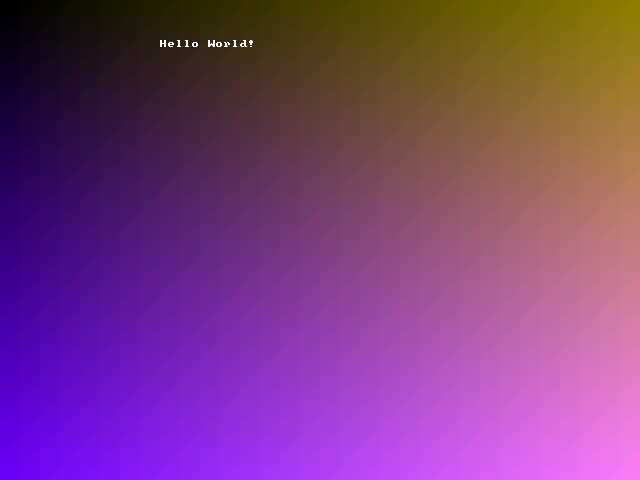
\includegraphics[width=5.5cm]{5} }}%
    \qquad
    \subfloat[\centering PS/2 driver test output]{{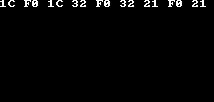
\includegraphics[width=8.6cm]{4} }}%
    \caption{}%
\end{figure}
\section{Reading Keyboard Input}
\subsection{PS/2 Driver}
To detect and read keystroke events through the PS/2 keyboard protocol, we create a PS/2 driver that inputs a memory address to store the data read from the PS/2 keyboard port if new data is available in the FIFO that stores data received from the PS/2 device.  We detect the availability of unread data by checking the $15^{th}$ (\verb+RVALID+) bit in the PS/2 data register. The subroutine returns the value of the \verb+RVALID+ bit.

This subroutine named \verb+read_PS2_data_ASM+ isolates the \verb+RVALID+ bit by performing an \verb+ANDS+ operation between the content of the PS/2 data register and 0x8000 (number only containing 1 as the 15th bit). If the \verb+RVALID+ bit is equal to 0, we store 0 in the return register \verb+R0+ and branch back to the caller. Otherwise, we read the first 8 bits of the PS/2 data register using a byte load operation (\verb+LDRB+) and store the loaded data into the address passed in the first argument R0 using \verb+STRB+. Finally, 1 is stored into \verb+R0+ before branching to the caller.

\subsection{Testing the PS/2 Driver}
To test the implemented PS/2 driver, we use the provided program that displays the make and break codes corresponding using the PS/2 keyboard device. We run the program and input the characters "a", "b", and "c" in sequence. The VGA display after performing this test is presented in Figure 1 (b). As shown in Figure 1 (b), 9 codes were printed on the VGA display. We can verify that the first, second, and third triplet corresponds to characters "a", "b", and "c" respectively. The first code in each triplet corresponds to the make code while the seconds and third codes together correspond to the break code. For instance, the first displayed triplet (\verb+1C F0 1C+) corresponds to character "a" with \verb+1C+ being the make code and \verb+F0 1C+ being the break code.
\section{Putting Everything Together: Vexillology}

\begin{figure}[h]
    \centering
    \subfloat[\centering Real-life flag (flag of Burkina Faso)]{{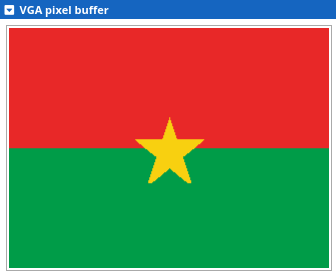
\includegraphics[width=4.9cm]{1} }}%
    \qquad
    \subfloat[\centering Imaginary flag]{{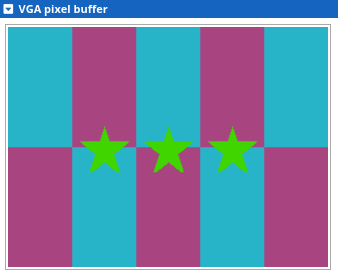
\includegraphics[width=4.9cm]{2} }}%
    \qquad
    \subfloat[\centering flag of Texas]{{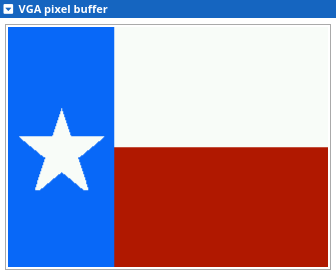
\includegraphics[width=4.9cm]{3} }}%
    \caption{}%
\end{figure}
\section{Conclusion}


\end{document}
